\chapter{Theory}
\label{Chap:theory}

% epigraph
\setlength{\unitlength}{1pt}
\setlength{\epigraphwidth}{10cm}
\epigraph{Law of physicists II: \\ Without theorists, experimentalists tend to falter.}{--- T.D. Lee\\ \textit{History of the weak interactions (1987)}}

% goal of this chapter and structure of this chapter
This chapter discusses two fundamental things: quantum scattering theory and theory of BEC-mixture qunautum droplet. first is the quantum scattering theory which is the basic for understanding the couple channel calculation in Chap. \ref{Chap_Feshbach}. The second part tries to describe the microscopic theory for a single BEC which serves as . We mainly introduce the beyond mean field thoery which will be used in the Chap. \ref{Chap_droplet} for a mixture of BEC to explain the droplet. We should noted here that the scattering properties stay at the core part to understand the behaviour of sample. More discussion about low dimensional scattering will be introduced in the last chaper and we will talk more about a low dimensional quantum gas and quantum droplet.

\section{Quantum scattering theory}
\label{sec:quan_scat}

We starting from the most general case, writing down a Bose system's Hamiltonian. Considering N spinless Bosons with mass m = 1 in volume V in 3-D space, and with thermal dynamic limit, i.e. N$\to \infty $ and V$\to
\infty $, and $\frac{N}{V}=n\to \text{finite}$), we write down the Hamiltonian
\begin{equation}
\begin{split}
\hat{H}_0&=\frac{1}{2}\int\nabla\hat{\Psi}^\dagger(x)\nabla\hat{\Psi }(x)dx=\frac{V}{(2\pi)^3}\int\epsilon_p^0\hat{a}_p^\dagger\hat{a}_pdp\\
\hat{H}_1&=\frac{1}{2}\int\hat{\Psi}^\dagger(x)\hat{\Psi}^\dagger(x')V(x-x')\hat{\Psi}(x')\hat{\Psi}(x)dxdx'=\frac{1}{2}\frac{V}{(2\pi)^3}\int V(p)\hat{a}_p^\dagger\hat{a}_{p'}^\dagger\hat{a}_{p'-q}\hat{a}_{p+q}dp
\end{split}
\end{equation}
with $\epsilon _p^0=\left.p^2\right/2$
For convenience we set $\hbar $ = 1.
where Fourier transformation for ladder operators are
\begin{equation}
\begin{split}
\hat{\Psi}(x)=\frac{1}{\sqrt{V}}\sum_{p}e^{ipx}\hat{a}_p=\frac{\sqrt{V}}{(2\pi)^3}\int dp e^{i p x}\hat{a}_p\\
\hat{\Psi}^\dagger(x)=\frac{1}{\sqrt{V}}\sum_p e^{-i p x}\hat{a}_p^\dagger=\frac{\sqrt{V}}{(2\pi)^3}\int dp e^{-i p x}\hat{a}_p^\dagger
\end{split}
\end{equation}
The interaction term $V(x-x')$ plays core role. Theoretically, it is hard to solve this problem because the real potential of atom-atom interaction is quite complicated. However, if we consider a special case, such that a bunch of Bose gas is quite dilute, we can use low-energy effective theory to tackle it.

There are three keywords for this special system: short-range interaction, dilute and low-temperature. 
Short-range gives a length scale $r_0$, which represent the inter-particle potential range. 
Dilute means: $n^{1/3}r_0<<1$, where n denote particle number density. 
Low temperature(energy) means $k r_0<<1$, where $k$ denotes momentum.

These three conditions allow us to ignore the complicated real potential between atoms, instead we can use scattering length (we will talk it later) to represent the whole scattering property of this system, especially at very low temperature left only one parameter, the s-wave scattering length $a_S$.

This note's material is arranged as following: first, we briefly talk about the basic scattering problem, which define $a_S$ in low temperature.
Then, we use mean field method solve Bose system, and discuss its ground state and excitation spectrum. Finally, we will go a little bit beyond the mean field theory, talking about quantum depletion and LHY correction.

\subsection{Scattering property}
The stationary Schrodinger equation and the Hamiltonian of the system is
\begin{equation}
\left(-\frac{\hbar ^2}{2m}\nabla ^2+\hat{V}(r)\right)\psi _k(r,\theta ,\phi )=\psi _k(r,\theta ,\phi )
\end{equation}
separating the state into radial and angular parts
\begin{equation}
\psi _k(r,\theta ,\phi )=R_l(k.r)Y_{\text{lm}}(\theta,\phi)
\end{equation}
and then the radial part equation
\begin{equation}
\left(\frac{d^2}{dr^2}+\frac{2}{r}\frac{d}{dr}-\frac{l(l+1)}{r^2}-\frac{2m}{\hbar ^2}V(r)+k^2\right)R_l(k,r)=0
\end{equation}
Then, we already know that the form of wave function when r is very large, i.e.
\begin{equation}
\psi (r)=e^{i k z}+f(k,\theta )\frac{e^{i k r}}{r}
\end{equation}
by spherical expanding we get:
For left side:
\begin{equation}
\psi (r)=\sum _{l =0}^{\infty } R_l(k,r)P_l(\text{Cos}[\theta ])
\end{equation}
For right side:
\begin{equation}
e^{i k z}=\sum _{l=0}^{\infty}(2l+1)i^l(kr)^{-1}\text{Sin}\left[k r-\frac{l \pi }{2}\right]P_l(\text{Cos}[\theta])
\end{equation}
\begin{equation}
f(k,\theta )=\sum _{l =0}^{\infty } f_l(k)P_l(\text{Cos}[\theta ])
\end{equation}
Thus we have the Radial part with different $l$ as
\begin{equation}
R_l(k,r)=(2l+1)i^l(k r)^{-1}\text{Sin}\left[k r-\frac{l \pi }{2}\right]+f_l(k)\frac{e^{i k r}}{r}
\end{equation}
Until now, we can only say that we find the connect between $R_l$ and $f_l$, however it doesn't help. But if we are treating some \pmb{finite range potential}, there exists a general solution:
Suppose that the potential can be written as
\begin{equation}
V(r)=\left\{
\begin{array}{c}
 V(r), r<r_0 \\
 0, r>r_0 \\
\end{array}
\right.
\end{equation}
When $r>r_0$ we have
\begin{equation}
\left(\frac{d^2}{dr^2}+\frac{2}{r}\frac{d}{dr}-\frac{l(l+1)}{r^2}+k^2\right)R_l(k,r)=0
\end{equation}
Solution of this equation has been solved well as following
\begin{equation}
R_l(k,r)=B_l(k)\text{SphericalBesselJ}[l,kr]+C_l(k)\text{SphericalBesselY}[l,\text{kr}]
\end{equation}
When r $\to \infty $, we get the asymptotic from of Bessel function as
\begin{equation}
R_l(k,r)=\frac{1}{k r}\left\{A_l(k)\text{Sin}\left[k r-\frac{l \pi }{2}-\delta _l(k)\right]\right\}
\end{equation}
where
\begin{equation}
A_l(k)=\sqrt{B_l^2(k)+C_l^2(k)},\text{  }\delta _l(k)=\text{ArcTan}\left[\frac{C_l(k)}{B_l(k)}\right]
\end{equation}
Comparing [12] and [16], we get that
\begin{equation}
f_l(k)=\frac{2l+1}{2i k}\left[e^{2i \delta _l(k)}-1\right]
\end{equation}
\begin{equation}
A_l(k)=(2l+1)i^le^{i \delta _l(k)}
\end{equation}
Finally, we have
\begin{equation}
f(k,\theta )=\sum _{l =0}^{\infty } \frac{2l+1}{2i k}\left[e^{2i \delta _l(k)}-1\right]P_l(\text{Cos}[\theta ])
\end{equation}
Now, if we connect the boundary condition inside $r_0$, we can totally solve out the $\delta _l(k)$ then solve out this problem.
For now, we can say that if we get all $\delta _l(k)$, then we solve this problems well. But that is a huge project because there are infinite $l$ and for each $l$, $\delta$ is a function of k, thus we need a good approximation for our system. Then, the last feature, low temperature, can be used. 
%\caption{Figure 1. For higher angular momentum $l$, it's hard to scatter with the short range hard core.}
As shown in figure, particles can hit this finite potential with $l$ less than 
\begin{equation}
l<l_{\max }=\frac{m v r_0}{\hbar }=r_0 k
\end{equation}
where $r_0$ is the potential range. Thus, At low-energy limit, i.e. $r_0k\to 0$, we have $l_{\max }\to 0$, which means we can consider S-wave only.
\begin{equation}
f_0(k)=\frac{1}{2ik}\left[e^{2i\delta_l(k)}-1\right]=\frac{1}{k}e^{i \delta _0(k)}\text{Sin}\left[\delta _0(k)\right]
\end{equation}
Thus, only one parameter $\delta _0(k)$ representing whole process. As historical preference, we introduce an equivalent parameter, scattering length $a_S$
\begin{equation}
a_s=a_0(k)|_{k\to0}=\underset{k\to0}{\text{Lim}}\left[-\frac{1}{k}\text{Tan}\left[\delta _0(k)\right]\right]
\end{equation}
where $a_s$ is independent with $k$, just as what we want.
Conclusion: when we deal with finite range potential scattering, not need to be finite intensity potential, and if the particle's momentum k is so small that $k<<\text{1/a}$, where a is the potential range, we can use only one parameter $a_0$ to describe the whole scattering process. The approximations made here are listed below:
Finite range potential gives $r_0$.
$k\ll 1\left/r_0 \right.$ where k is scattering momentum divided by $\hbar$, and $r_0$ is potential range
Scattering length $a_0$ actually depends on k, however if we consider the limit $k\to 0$, we can ignore this variance.
This very beautiful property gives us a way to deal with not-weak atom-atom scattering problem even with strong interaction.

\subsection{Basic theory of Double BEC}
Now, we turn to describe double BEC with mean field theory, which will be used in Bose mixture droplet in journal club.
\subsection{Pseudo-Hamiltonian and extended Bogoliubov transformation}
Hamiltonian for BEC with two species is
\begin{equation}
H_{\text{tot}}=\sum_k\epsilon_{1,k}\hat{a}_{1,k}\dagger\hat{a}_{1,k}+\frac{g_{11}}{2V}\sum_{\left\{k_i\right\}}\hat{a}_{1,k_1}^+\hat{a}_{1,k_2}^+\hat{a}_{1,k_3}\hat{a}_{1,k_4}+\sum_k\epsilon_{2,k}\hat{a}_{2,k}\dagger\hat{a}_{2,k}+\frac{g_{22}}{2V}\sum_{\left\{k_i\right\}}\hat{a}_{2,k_1}^+\hat{a}_{2,k_2}^+\hat{a}_{2,k_3}\hat{a}_{2,k_4}+\frac{g_{12}}{V}\sum_{\left\{k_i\right\}}\hat{a}_{2,k_1}^+\hat{a}_{1,k_2}^+\hat{a}_{1,k_3}\hat{a}_{2,k_4}
\end{equation}
where $k_1+k_2=k_3+k_4$, satisfy momentum conservation.$g_{\text{ii}}$ represent intra-interaction strength, and $g_{12}$ for inter-interaction.
$\hat{a}_{i,k}^+$($\hat{a}_{i,k}$) denote the ladder operator for $i^{\text{th}}$ component.
Because of the special role of the state with k = 0, i.e. condensate, we separate ladder operator into two piece for whole Bose gas
\begin{equation}
\hat{\Psi }_i(x)=\frac{1}{\sqrt{V}}\sum_{p\neq0}e^{ipx}\hat{a}_{i,p}+\frac{1}{\sqrt{V}}\hat{a}_{i,0}=\hat{\Psi }_i'(x)+\frac{1}{\sqrt{V}}\hat{a}_{i,0}
\end{equation}
\begin{equation}
\hat{\Psi }_i\dagger(x)=\frac{1}{\sqrt{V}}\sum_{p\neq0}e^{-ipx}\hat{a}_{i,p}\dagger+\frac{1}{\sqrt{V}}\hat{a}_{i,0}\dagger=\hat{\Psi}'\dagger(x)+\frac{1}{\sqrt{V}}\hat{a}_{i,0}\dagger
\end{equation}
Then we get Hamiltonian as
\begin{equation}
\begin{split}
H=\frac{g_{11}N_1^2+g_{22}N_2^2+2g_{12}N_1N_2}{2V}+\sum _{k\neq 0} \left(\epsilon _{1,k}+\frac{g_{11}N_1+g_{12}N_2}{V}\right)\hat{a}_{1,k}\dagger\hat{a}_{1,k}+\sum_{k\neq 0} \left(\epsilon _{2,k}+\frac{g_{22} N_2+g_{12}N_1}{V}\right)\hat{a}_{2,k}\dagger\hat{a}_{2,k}+\\
\frac{g_{11} N_1}{2V}\sum _{k\neq 0} \left(\hat{a}_{1,k}^+\hat{a}_{1,-k}^++\hat{a}_{1,k}\hat{a}_{1,-k}\right)+\frac{g_{22} N_2}{2V}\sum_{k\neq0}\left(\hat{a}_{2,k}^+\hat{a}_{2,-k}^++\hat{a}_{2,k}\hat{a}_{2,-k}\right)+\frac{g_{12}\sqrt{N_1N_2}}{2V}\sum _{k\neq 0} \left(\hat{a}_{1,k}^+\hat{a}_{2,k}+\hat{a}_{2,k}^+\hat{a}_{1,k}+\hat{a}_{1,k}\hat{a}_{2,-k}+\hat{a}_{2,k}^+\hat{a}_{1,-k}^+\right)
\end{split}
\end{equation}
where we only keep the second order of $N_i$, dropping third and forth order of $N_i$. Then, diagonalize this Hamiltonian by extended Bogoliubov transformation for double BEC, we have
\begin{equation}
H=\frac{g_{11}N_1^2+g_{22}N_2^2+2g_{12}N_1N_2}{2V}+\frac{1}{2}\sum _{k\neq 0} \left(E_++E_--\frac{\hbar ^2k^2}{2m_1}-\frac{\hbar ^2k^2}{2m_2}-\frac{g_{11}N_1+g_{22}N_2}{V}\right)+\sum_{k\neq 0} E_{+,k}\hat{a}_{+,k}\dagger\hat{a}_{+,k}+\sum _{k\neq 0} E_{-,k}\hat{a}_{-,k}\dagger\hat{a}_{-,k}
\end{equation}
where
\begin{equation}
E_{\pm }=\sqrt{\frac{\omega _1^2+\omega _2^2}{2}\pm \sqrt{\left(\frac{\omega _1^2-\omega _2^2}{2}\right){}^2+\frac{g_{12}^2N_1N_2}{V^2}\frac{\hbar
^2k^4}{m_1m_2}}}
\end{equation}
where
\begin{equation}
\omega _i=\sqrt{\frac{\hbar ^2k^2}{2m_i}\left(\frac{\hbar ^2k^2}{2m_i}+\frac{2g_{\text{ii}}N_i}{V}\right)}
\end{equation}
We plot the spectrum for each channel $E_+$ and $E_-$, with $\text{$\delta $g}=\sqrt{g_{11}g_{22}}-g_{12}>0$ and $\text{$\delta $g}=\sqrt{g_{11}g_{22}}-g_{12}<0$
Where we find similar spectrum with one component BEC. For $\text{$\delta $g}<0$, we get complex energy with small $k$, which represent unstable of the system.

\subsection{Ground state energy and LHY correction}
Ground state energy will be
\begin{equation}
E_{\text{GS}}=\frac{g_{11}N_1^2+g_{22}N_2^2+2g_{12}N_1N_2}{2V}+\frac{1}{2}\sum _{k\neq0}\left(E_++E_--\frac{\hbar^2k^2}{2m_1}-\frac{\hbar ^2k^2}{2m_2}-\frac{g_{11}N_1+g_{22}N_2}{V}\right)
\end{equation}
After re-normalization we have
\begin{equation}
E_{\text{GS}}^R=\frac{g_{11}N_1^2+g_{22}N_2^2+2g_{12}N_1N_2}{2V}+\frac{1}{2}\sum _{k\neq 0} \left(E_++E_--\frac{\hbar ^2k^2}{2m_1}-\frac{\hbar^2k^2}{2m_2}-\frac{g_{11}N_1+g_{22}N_2}{V}+\frac{m_1g_{11}^2N_1^2/V^2+m_2g_{22}^2N_2^2/V^2+4\frac{m_1m_2}{m_1+ m_2}g_{12}^2N_1N_2/V^2}{\hbar ^2k^2}\right)
\end{equation}
The second term is LHY term which can be rewritten as
\begin{equation}
E_{\text{LHY}}=\frac{1}{2}\sum _{k\neq0}\left(\sqrt{\frac{\omega _1^2+\omega _2^2}{2}+\sqrt{\left(\frac{\omega_1^2-\omega_2^2}{2}\right){}^2+g_{12}^2n_1n_2\frac{\hbar^4k^4}{m_1m_2}}}+\sqrt{\frac{\omega _1^2+\omega_2^2}{2}-\sqrt{\left(\frac{\omega_1^2-\omega _2^2}{2}\right){}^2+g_{12}^2n_1n_2\frac{\hbar^4k^4}{m_1m_2}}}-\frac{\hbar^2k^2}{2m_1}-\frac{\hbar^2k^2}{2m_2}-g_{11}n_1-g_{22}n_2+\frac{m_1g_{11}^2n_1^2+m_2g_{22}^2n_2^2+4\frac{m_1m_2}{m_1+m_2}g_{12}^2n_1n_2}{\hbar ^2k^2}\right)
\end{equation}
into integral formation
\begin{equation}
\frac{E_{\text{LHY}}}{V}=\int _0^{k_c}\frac{k^2}{4\pi ^2}\left(\sqrt{\frac{\omega_1^2+\omega_2^2}{2}+\sqrt{\left(\frac{\omega_1^2-\omega_2^2}{2}\right){}^2+g_{12}^2n_1n_2\frac{\hbar^4k^4}{m_1m_2}}}+\sqrt{\frac{\omega_1^2+\omega_2^2}{2}-\sqrt{\left(\frac{\omega_1^2-\omega_2^2}{2}\right){}^2+g_{12}^2n_1n_2\frac{\hbar^4k^4}{m_1m_2}}}-\frac{\hbar^2k^2}{2m_1}-\frac{\hbar^2k^2}{2m_2}-g_{11}n_1-g_{22}n_2+\frac{m_1g_{11}^2n_1^2+m_2g_{22}^2n_2^2+4\frac{m_1m_2}{m_1+ m_2}g_{12}^2n_1n_2}{\hbar ^2k^2}\right)dk
\end{equation}
\begin{equation}
\begin{split}
\frac{E_{\text{LHY}}}{V}=C_1\int _0^{k_c}\frac{\tilde{k}^2}{4\pi ^2}\left(\sqrt{\frac{1}{2}\left(\frac{\tilde{k}^2}{2}\left(\frac{\tilde{k}^2}{2}+2\right)+\frac{1}{\gamma^2}\frac{\tilde{k}^2}{2}\left(\frac{\tilde{k}^2}{2}+2y\gamma\right)\right)+\sqrt{\left(\frac{1}{2}\left(\frac{\tilde{k}^2}{2}\left(\frac{\tilde{k}^2}{2}+2\right)-\frac{1}{\gamma^2}\frac{\tilde{k}^2}{2}\left(\frac{\tilde{k}^2}{2}+2y \gamma \right)\right)\right)^2+\frac{xy}{\gamma }\tilde{k}^4}}+\right.\\
\left.\sqrt{\frac{1}{2}\left( \frac{\tilde{k}^2}{2}\left(\frac{\tilde{k}^2}{2}+2\right)+\frac{1}{\gamma ^2}\frac{\tilde{k}^2}{2}\left(\frac{\tilde{k}^2}{2}+2y\gamma \right)\right)-\sqrt{\left(\frac{1}{2}\left(\frac{\tilde{k}^2}{2}\left(\frac{\tilde{k}^2}{2}+2\right)-\frac{1}{\gamma ^2}\frac{\tilde{k}^2}{2}\left(\frac{\tilde{k}^2}{2}+2y\gamma \right)\right)\right)^2+\frac{xy}{\gamma}\tilde{k}^4}}-\frac{\tilde{k}^2}{2}\left(1+\frac{1}{\gamma }\right)-1-y+\frac{1+\gamma y^2+\frac{4xy \gamma}{1+\gamma}}{\tilde{k}^2}\right)d\tilde{k}
\end{split}
\end{equation}

\begin{equation}
\begin{split}
C_1=g_{11}n_1\left(\frac{\sqrt{m_1g_{11}n_1}}{\hbar }\right){}^3\\
\gamma =\frac{m_2}{m_1}\\
x=\frac{g_{12}^2}{g_{11}g_{22}}\\
y=\frac{g_{22}n_2}{g_{11}n_1}\\
\tilde{k}=\frac{\hbar  k}{\sqrt{m_1g_{11}n_1}}
\end{split}
\end{equation}
\begin{equation}
\frac{\omega _1}{g_{11}n_1}=\sqrt{\frac{\hbar^2k^2}{2m_1g_{11}n_1}\left(\frac{\hbar^2k^2}{2m_1g_{11}n_1}+2\right)}=\sqrt{\frac{\tilde{k}^2}{2}\left(\frac{\tilde{k}^2}{2}+2\right)}
\end{equation}
\begin{equation}
\frac{\omega _2}{g_{11}n_1}=\sqrt{\frac{\hbar^2k^2}{2m_2g_{11}n_1}\left(\frac{\hbar^2k^2}{2m_2g_{11}n_1}+2\frac{g_{22}n_2}{g_{11}n_1}\right)}=\sqrt{\frac{1}{\gamma}\frac{\tilde{k}^2}{2}\left(\frac{1}{\gamma}\frac{\tilde{k}^2}{2}+2y\right)}=\frac{1}{\gamma}\sqrt{\frac{\tilde{k}^2}{2}\left(\frac{\tilde{k}^2}{2}+2y\gamma \right)}
\end{equation}
we take out the dimensionless part of it, i.e.
\begin{equation}
E_{\text{GS}}^R=\frac{g_{11}N_1^2+g_{22}N_2^2+2g_{12}N_1N_2}{2V}+\frac{8V}{15\pi^2}m_1^{3/2}\left(g_{11}n_1\right){}^{5/2}f\left(\frac{m_2}{m_1},\frac{g_{12}^2}{g_{11}g_{22}},\frac{g_{22}n_2}{g_{11}n_1}\right)
\end{equation}
Where $f$ is always larger than 0 and is dimensionless.
We will show in this week's journal club that, the second term of LHY correction will actually stabilize the system from collapse and will not require entering strong interaction regime.

\begin{equation}
\frac{1}{2}\left(
\begin{array}{cc}
 n_1 & n_2 \\
\end{array}
\right)\left(
\begin{array}{cc}
 g_{11} & g_{12} \\
 g_{12} & g_{22} \\
\end{array}
\right)\left(
\begin{array}{c}
 n_1 \\
 n_2 \\
\end{array}
\right)
\end{equation}
diagonalize
\begin{equation}
\lambda _+=\frac{g_{11}+g_{22}}{2},\lambda_-=\frac{\sqrt{g_{11}g_{22}}}{g_{11}+g_{22}}\text{$\delta $g}
\end{equation}
\begin{equation}
n_+=\frac{n_1\sqrt{g_{11}}-n_2\sqrt{g_{22}}}{\sqrt{g_{11}+g_{22}}}, n_-=\frac{n_1\sqrt{g_{22}}+n_2\sqrt{g_{11}}}{\sqrt{g_{11}+g_{22}}}
\end{equation}

\subsection{Scattering in low dimension}
\subsection{Resonance scattering}






% from intro about the LHY correction and quantum depletion

\subsection{Dilute Bose system: Pseudo-Hamiltonian and Bogoliubov transformation}
As we can use $a_S$ representing scattering process, we can write down a pseudo-potential, which gives the same effect as the original one. This procedure first done by \textit{Fermi} as following
\begin{equation}
V(r)=g \delta (r)\partial _r\cdot r=\frac{4\pi\hbar^2a_S}{m}\delta (r)\partial _r\cdot r
\end{equation}
which is a contact potential only affect two atoms when they have same $r$. The last term $\partial _r\cdot r$ eliminates wave function's divergence at $r\to 0$, due to it has form of $\psi \to 1-\left.a_S\right/r$. if we write the potential as
\begin{equation}
V(r)=g_R\delta (r)
\end{equation}
where $g_R$ denotes the interaction intensity. Note that this $g_R$ cannot be considered as physics quantity due to its divergence at $r\to 0$. However, the relationship between $g_R$ and $g$ can be obtain by \textit{Dyson} Equation.
\begin{equation}
g_R=g+g \Sigma ^* g_R
\end{equation}
where $g_R$ represent normalized interaction strength, and $\Sigma$ represent the proper self-energy of system, i.e.
\begin{equation}
g_R=\frac{4\pi  \hbar ^2a_S}{m}\left(1+\frac{g_R}{V}\sum _{k=0}^{\infty } \frac{1}{\hbar ^2\left.k^2\right/m}\right)
\end{equation}
by just take the second order correction (loop correction), we get
\begin{equation}
g_R=g\left(1+\frac{g}{V}\sum _{k=0}^{\infty } \frac{1}{\hbar ^2\left.k^2\right/m}\right)
\end{equation}
The second term is actually diverge, which represents high energy scattering. This term will only be used when we need to sum over some term with all high energy collision process. In most time, we can just take $g$ as
\begin{equation}
g=\frac{4\pi  \hbar ^2a_S}{m}
\end{equation}
Then, we can rewrite the whole Hamiltonian as following
\begin{equation}
\begin{split}
\hat{H}_0&=\frac{1}{2}\int \nabla \hat{\Psi }\dagger(x)\nabla \hat{\Psi }(x)dx\\
H_1&\simeq \frac{1}{2}\int \hat{\Psi }\dagger(x)\hat{\Psi }\dagger(x')g \delta (x-x')\hat{\Psi }(x')\hat{\Psi }(x)dxdx'=\frac{g}{2}\int \hat{\Psi}\dagger(x)\hat{\Psi }\dagger(x)\hat{\Psi }(x)\hat{\Psi }(x)dx
\end{split}
\end{equation}
Fourier transformation gives the Hamiltonian in momentum space as
\begin{equation}
H_{\text{pseudo}}=\sum_k\epsilon_k\hat{a}_k\dagger\hat{a}_k+\frac{g}{2V}\sum _{\left\{k_i\right\}}\hat{a}_{k_1}^+\hat{a}_{k_2}^+\hat{a}_{k_3}\hat{a}_{k_4}
\end{equation}
where $k_1+k_2=k_3+k_4$, satisfies momentum conservation. This is just the pseudo-Hamiltonian for many-Boson system.
Because of the special role of the state with k = 0, i.e. condensate, we separate ladder operator into two piece for whole Bose gas
\begin{equation}
\hat{\Psi }(x)=\frac{1}{\sqrt{V}}\sum _{p\neq 0} e^{i p x}\hat{a}_p+\frac{1}{\sqrt{V}}\hat{a}_0=\hat{\Psi }'(x)+\frac{1}{\sqrt{V}}\hat{a}_0
\end{equation}
\begin{equation}
\hat{\Psi }\dagger(x)=\frac{1}{\sqrt{V}}\sum _{p\neq 0} e^{-i p x}\hat{a}_p\dagger+\frac{1}{\sqrt{V}}\hat{a}_0\dagger=\hat{\Psi }'\dagger(x)+\frac{1}{\sqrt{V}}\hat{a}_0\dagger
\end{equation}
where $\hat{a}_0=\hat{a}_0\dagger=\sqrt{n}=\sqrt{\frac{N}{V}}$
notice that {``}mean field{''} just means taking some quantum operator as a c-number, which is average of this operator, so the quantum fluctuation is blurred. So, when we use mean field theory to calculate the system ,we need pay attention to what fluctuation we take it from the calculation, then at necessary time, we can get it back.
put them into (31), then simply
\begin{equation}
\begin{split}
H=\frac{g N^2}{2V}&+\sum_{k\neq0}\left(\epsilon_k+gn_0\right)\hat{a}_k\dagger\hat{a}_k+\frac{gN}{2V}\sum_{k\neq0}\left(\hat{a}_k^+\hat{a}_{-k}^++\hat{a}_k\hat{a}_{-k}\right)\\
&+\frac{g\sqrt{N}}{2V}\sum_{k_1+k_2+k_3=0}\left(\hat{a}_{k_1}^+\hat{a}_{k_2}^+\hat{a}_{k_3}+\hat{a}_{k_1}^+\hat{a}_{k_2}\hat{a}_{k_3}\right)+\frac{g}{2V}\sum_{k_i\neq0}\hat{a}_{k_1}^+\hat{a}_{k_2}^+\hat{a}_{k_3}\hat{a}_{k_4}
\end{split}
\end{equation}
Here, we drop the terms with N's order less than $N$, because they became very smaller than formers when temperature is quite low that large amount of atoms are condensate. (If considering the last two term, we will get the Beliaev-Landau Damping.)
\begin{equation}
H_{\text{pseudo}}\simeq\frac{gN^2}{2V}+\sum_{k\neq0}\left(\epsilon _k+g n_0\right)\hat{a}_k\dagger\hat{a}_k+\frac{gn_0}{2}\sum_{k\neq0}\left(\hat{a}_k^+\hat{a}_{-k}^++\hat{a}_k\hat{a}_{-k}\right)\end{equation}
Now, as quadratic form, we can diagonalize it with so called Bogoliubov transformation
\begin{equation}
\begin{split}
\hat{a}_k=u_k\hat{\alpha }_k-v_k\alpha _{-k}^+\\
\hat{a}_{-k}=u_k\hat{\alpha }_{-k}-v_k\alpha _k^+
\end{split}
\end{equation}
where $\alpha _k^+\left(\alpha _k\right)$ is a new ladder operator, which actually denote create(annihilate) a quasi-particle in this condensate system. $u_k$ and $v_k$ is c-number as function of $k$ and $E_k$, which gives the spectrum of quasi-particle. 
Finally, we give out the diagonalized Hamiltonian as
\begin{equation}
\begin{split}
H_{\text{pseudo}}\simeq \frac{g N^2}{2V}-\frac{1}{2}\sum _{k\neq 0} \left(\epsilon _k+\frac{g N}{V}-E_k\right)+\sum _{k\neq 0} E_k\hat{\alpha }_k\dagger\hat{\alpha
}_k\\
E_k=\sqrt{\epsilon _k\left(\epsilon _k+\frac{2 g N}{V}\right)}=\sqrt{\frac{\hbar ^2k^2}{2m}\left(\frac{\hbar ^2k^2}{2m}+\frac{2 g N}{V}\right)}
\end{split}
\end{equation}
%Here needs a figure
%\caption{Figure 2. This plot shows the dissipation relation ship for quasi-particle in the Bose-condensation. When k is small, it looks like a phonon, however, when k goes large it back to a particle-like quasi-particle.}
Note that the gap-less linear low energy excited dissipation relation gives the super fluid property. when $k$ get larger, it turn back to classical particle.
Now, let's consider what happens when $g<0$, i.e. attractive potential between atoms. The excitation spectrum will be
%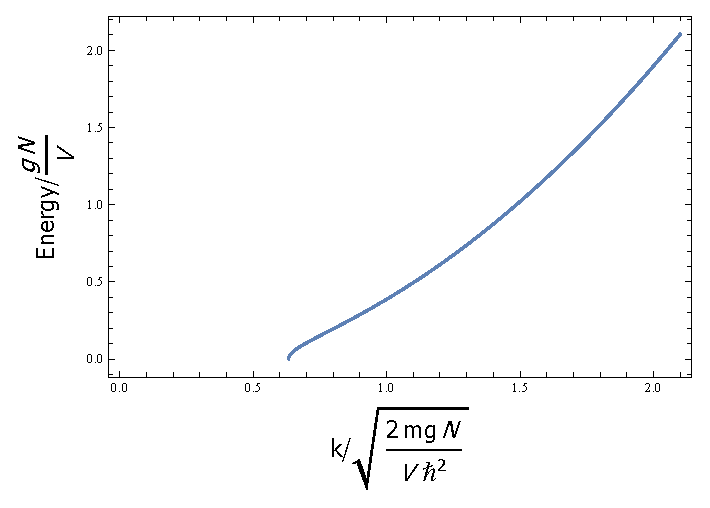
\includegraphics{Note for review_gr2.eps}
%\caption{Figure 3. This plot shows the dissipation relationship for attractive Bose-system.}
We find no excitation for small $k$, which means ground state has non-zero momentum, violating our assumption that condensate stay at $k=0$.
Thus, this result actually tells us that this attractive Bose-gas can not exist stable. We will return to this point later, when we talk about the ground state energy of this Bose system and also for double BEC case.

\subsection{Ground state and LHY correction}
Now we consider the ground state of this system. Directly take the lowest energy level from (38), we have
\begin{equation}
\begin{split}
E_{\text{GS}}=\frac{g N^2}{2V}-\frac{1}{2}\sum _{k\neq 0} \left(\epsilon _k+\frac{g N}{V}-E_k\right)
\end{split}
\end{equation}
where first term represent the mean field energy shift from {``}vacuum{''}, and second term come from quantum fluctuation (at zero temperature), i.e.
\begin{equation}
-\frac{1}{2}\sum _{k\neq 0} \left(\epsilon _k+\frac{g N}{V}-E_k\right)=-\frac{1}{2}\sum _{k\neq 0} \left(\frac{\hbar ^2k^2}{2m}+\frac{g N}{V}-\sqrt{\frac{\hbar
^2k^2}{2m}\left(\frac{\hbar ^2k^2}{2m}+\frac{2 g N}{V}\right)}\right)
\end{equation}
If you plot the term in the summation, you will find it decays with k increasing. However, if we expand it in series, we have 
\begin{equation}
\begin{split}
\frac{\hbar ^2k^2}{2m}&+\frac{g N}{V}-\sqrt{\frac{\hbar ^2k^2}{2m}\left(\frac{\hbar ^2k^2}{2m}+\frac{2 g N}{V}\right)}\\
&=\frac{1}{2}\left(\frac{gN}{V}\right)^2\left(\frac{2m}{\hbar^2}\right)\frac{1}{\pmb{k^2}}-\frac{1}{2}\left(\frac{gN}{V}\right)^3\left(\frac{2m}{\hbar^2}\right)^2\frac{1}{\pmb{k^4}}+\frac{5}{8}\left(\frac{gN}{V}\right)^4\left(\frac{2m}{\hbar^2}\right)^3\frac{1}{\pmb{k^6}}+\text{...}
\end{split}
\end{equation}
with leading proportional to $\frac{1}{k^2}$, we have divergence when sum over k to infinite. This divergence is due to the pseudo-potential with $\delta (r)$ actually does not allow calculation for large $k$, thus, we need do re-normalization to truncate this $\frac{1}{k^2}$ divergence.
Recalling the re normalized interaction $g_R$ in (27), we have
\begin{equation}
g_R=g+\frac{g^2}{V}\sum _k \frac{m}{\hbar ^2k^2}
\end{equation}
Then total energy will be
\begin{equation}
E_{\text{GS}}^R=\frac{gN^2}{2V}-\frac{1}{2}\sum_{k\neq0}\left(\frac{\hbar ^2k^2}{2m}+\frac{gN}{V}-\sqrt{\frac{\hbar^2k^2}{2m}\left(\frac{\hbar^2k^2}{2m}+\frac{2gN}{V}\right)}-\left(\frac{gN}{V}\right)^2\left(\frac{2m}{\hbar ^2}\right)\frac{1}{k^2}\right)
\end{equation}
Directly do this summation, we get the famous LHY correction
\begin{equation}
\frac{E_{\text{GS}}^R}{V}=\frac{g n^2}{2}\left(1+\frac{128}{15\pi ^{1/2}} \left(n a^3\right)^{1/2}\right)
\end{equation}
where $a=\text{Abs}\left[a_S\right]$. Now, we plot ground state energy when $g>0$
Where we can find the LHY correction is small when density is low, and only get important when $n a^3\sim 1$. These correction has been experimentally verified in strong interacting Bose System [PRL 107, 135301].
Then we plot the ground state energy with $g<0$
%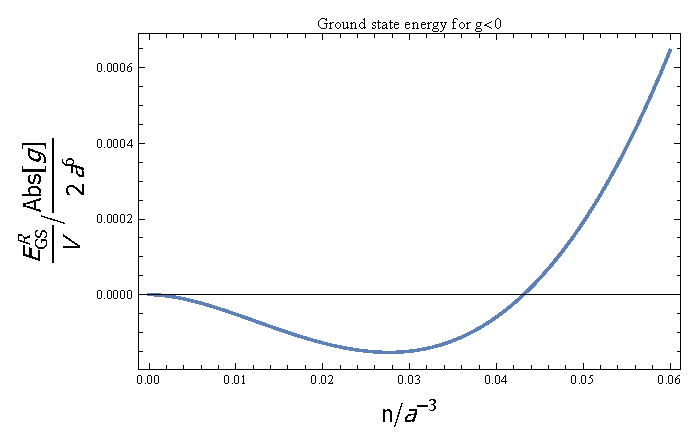
\includegraphics{Note for review_gr3.eps}
Where we find that only when \begin{equation}n a^3>0.028\end{equation}, the ground state energy increase with n increasing, which means stable ground state exist. This stability is reached due to quantum fluctuation resisting the collapse from attractive interacting, which has the same mechanics of liquid droplet in which stability is reached due to Van de Waals force. This so called LHY droplet seems haven{'}t been observed in experiment, I guess main reason is when $n a^3$ get large, the many body loss will be severe, which hides the phenomenon of droplet. We will talk more about the mechanics of LHY droplet when we considering the quantum depletion.

\subsection{Quantum Depletion and Mechanism of LHY Droplet}
Let's now consider: in a ground state of BEC at zero temperature, how many particles will not stay at $k=0$ state? The answer is just directly summation all non-zero k state in the ground state. as following
\begin{equation}
n_{\text{dp}}=\frac{1}{V}\sum _{k\neq 0} v_k^2=\frac{1}{3\pi ^2}\left(\frac{m c}{\hbar }\right)^3\propto \xi ^{-3}
\end{equation}
where $v_k$ is parameter in Bogoliubov transformation, $c =\sqrt{\frac{g n}{2m}}$ is the first sound speed in BEC, and $\xi =\frac{\hbar }{\sqrt{2m g n}}$ is healing length.
The fraction of depleted particle is
\begin{equation}
\frac{n_{\text{dp}}}{n}=\frac{8}{3\sqrt{\pi }}\sqrt{n a_S^3}
\end{equation}
we can directly read that with increasing of $n a_S^3$, more particles get out of the condensate. Meanwhile, these particles will contribute the LHY correction to ground state energy. Thus, we find that this correction beyond mean field theory actually always increase the energy and also increase {``}hot{''} particles. Moreover, if you consider the excitation spectrum for $g<0$, you can explain that the high energy excitation(short-wave)
actually cure the unstable system from long-wave-instability, which gives the formation of LHY droplet.

%For a single species condensate, with the mean-field approximation, we have its energy density propotional to \(n^2\). This is valid for low density case, which satisfies \(na_s^3<<1\). When the condition is brocken, we need a correction to further describe its behaviour, i.e. the LHY correction. From the view of ground state energy, this correction is with order of \(na_s^3\) comparing to the mean-field part, which in most case is too weak to detect. 
%这里从历史角度出发,谈历史上是如何测量LHY correction的

% discuss quantum depletion in this part
%From another point of view, i.e. how many particle stay beyond the zero momentum state, we need to introduce the quantum depletion. Similar to thermal depletion of a condensate, the quantum depletion is excited due to the inter-particle interaction. The depletion density can be written as




\chapterend

